% !TEX root =  main.tex

\section{Additional details pertaining to cancer simulator}
\label{sec:cancer_sim_app}

In this section, we elucidate some more details about the cancer simulator described in the manuscript, provide more rigorous mathematical definitions for the relevant terms using the same nomenclature, and also include more results figures.

\subsection{Simulator details}
\label{sec:cancer_sim_details}

We define $I(T_{\text{treat}})$ to be the expected proportion of patients who receive treatment.
A particular patient is represented by $y\in\mathcal{R}^d$. Specifically, $y$ consists of only a single real number ($d=1$) representing the size of the tumor upon discovery. Initial tumor size is drawn from a scaled Rayleigh distribution.
The outcome of the simulator is then $\phi(y,z)\in\left\lbrace 0,1\right\rbrace $, and is the binary outcome of whether that particular patient and sample of unobserved parameters yield an expected tumor size below the threshold, $T_{opp}$, after a fixed time duration, $t_{max}$. The simulator is a pair of coupled, parameterized differential equations for the action of an anti-tumor treatment such as chemotherapy, as described in~\citet{enderling2014cancer}:
\begin{align}
&\frac{dc}{dt} = -\lambda c \log\big(\frac{c}{K}\big) - \xi c \\
&\frac{dK}{dt} = \phi c - \psi K c^{2/3},
\end{align}
where $c(t,x)\in\mathcal{R}_+$ represents tumor size, with initial size $y_n$.
Similarly, $K(t,x)\in\mathcal{R}_+$ represents the notion of a carrying capacity, with the initial carrying capacity, $K(0,z)$, set to a known constant $K_0$.
The magnitude of the patient response to an anti-tumor treatment (such as chemotherapy) is represented by $\xi\in[0,1]$, drawn from a beta distribution.
$\{\lambda, \psi, \phi\}\in\mathcal{R}_+^3$ represent the parameters of the simulator.
We also define $x _{n,m}= \{\lambda, \psi, \phi\, K_0, \xi\}$ and $z_{n,m}=\{x_{n,m}, T_{\text{opp}}, t_{\text{max}}\}$, where all but £$\xi$ are set to constant values. Expanding this to condition all values on $y_n$ is trivial given domain knowledge. Alternatively, they could also be drawn at random, but not be conditioned on $y_n$. Such relations are omitted here for simplicity.

We can now fully define $\phi$ as:
\begin{equation}
\phi(y_n,z_{n,m}) = \mathbbm{1}(c(t_{\text{max}}, x_{n,m})<T_{\text{opp}}).
\end{equation}
Taking the expectation of $\phi$ over $M$ different realizations of $z$ yields the estimate $(\hat{\gamma}_M)_n$. 
This value is the probability that treatment will be successful for a particular patient, marginalizing over possible unobserved dynamics. This is the point at which clinician decides whether initiate the treatment plan.
This decision is represented $f(y_n,(\hat{\gamma}_M)_n) \in [0,1]$ as:
\begin{equation}
f(y_n,(\hat{\gamma}_M)_n) = \mathbbm{1}((\hat{\gamma}_M)_n>T_{\text{treat}})
\end{equation}
where $T_{\text{treat}}$ is the minimum probability of success required for that patient to receive the treatment, and again, could be conditioned on $y$ also.
Taking the expectation of $f$ over patients yields the expected frequency with which the treatment will be delivered, given a value of $T_{\text{treat}}$. The hospital wishes to estimate the value $T_{\text{treat}}$ that maximizes the number of patients treated, while only treating those patients with the highest probability of success, and (in expectation) staying within the budgetary constraint.

\begin{figure}[t]
	\centering
	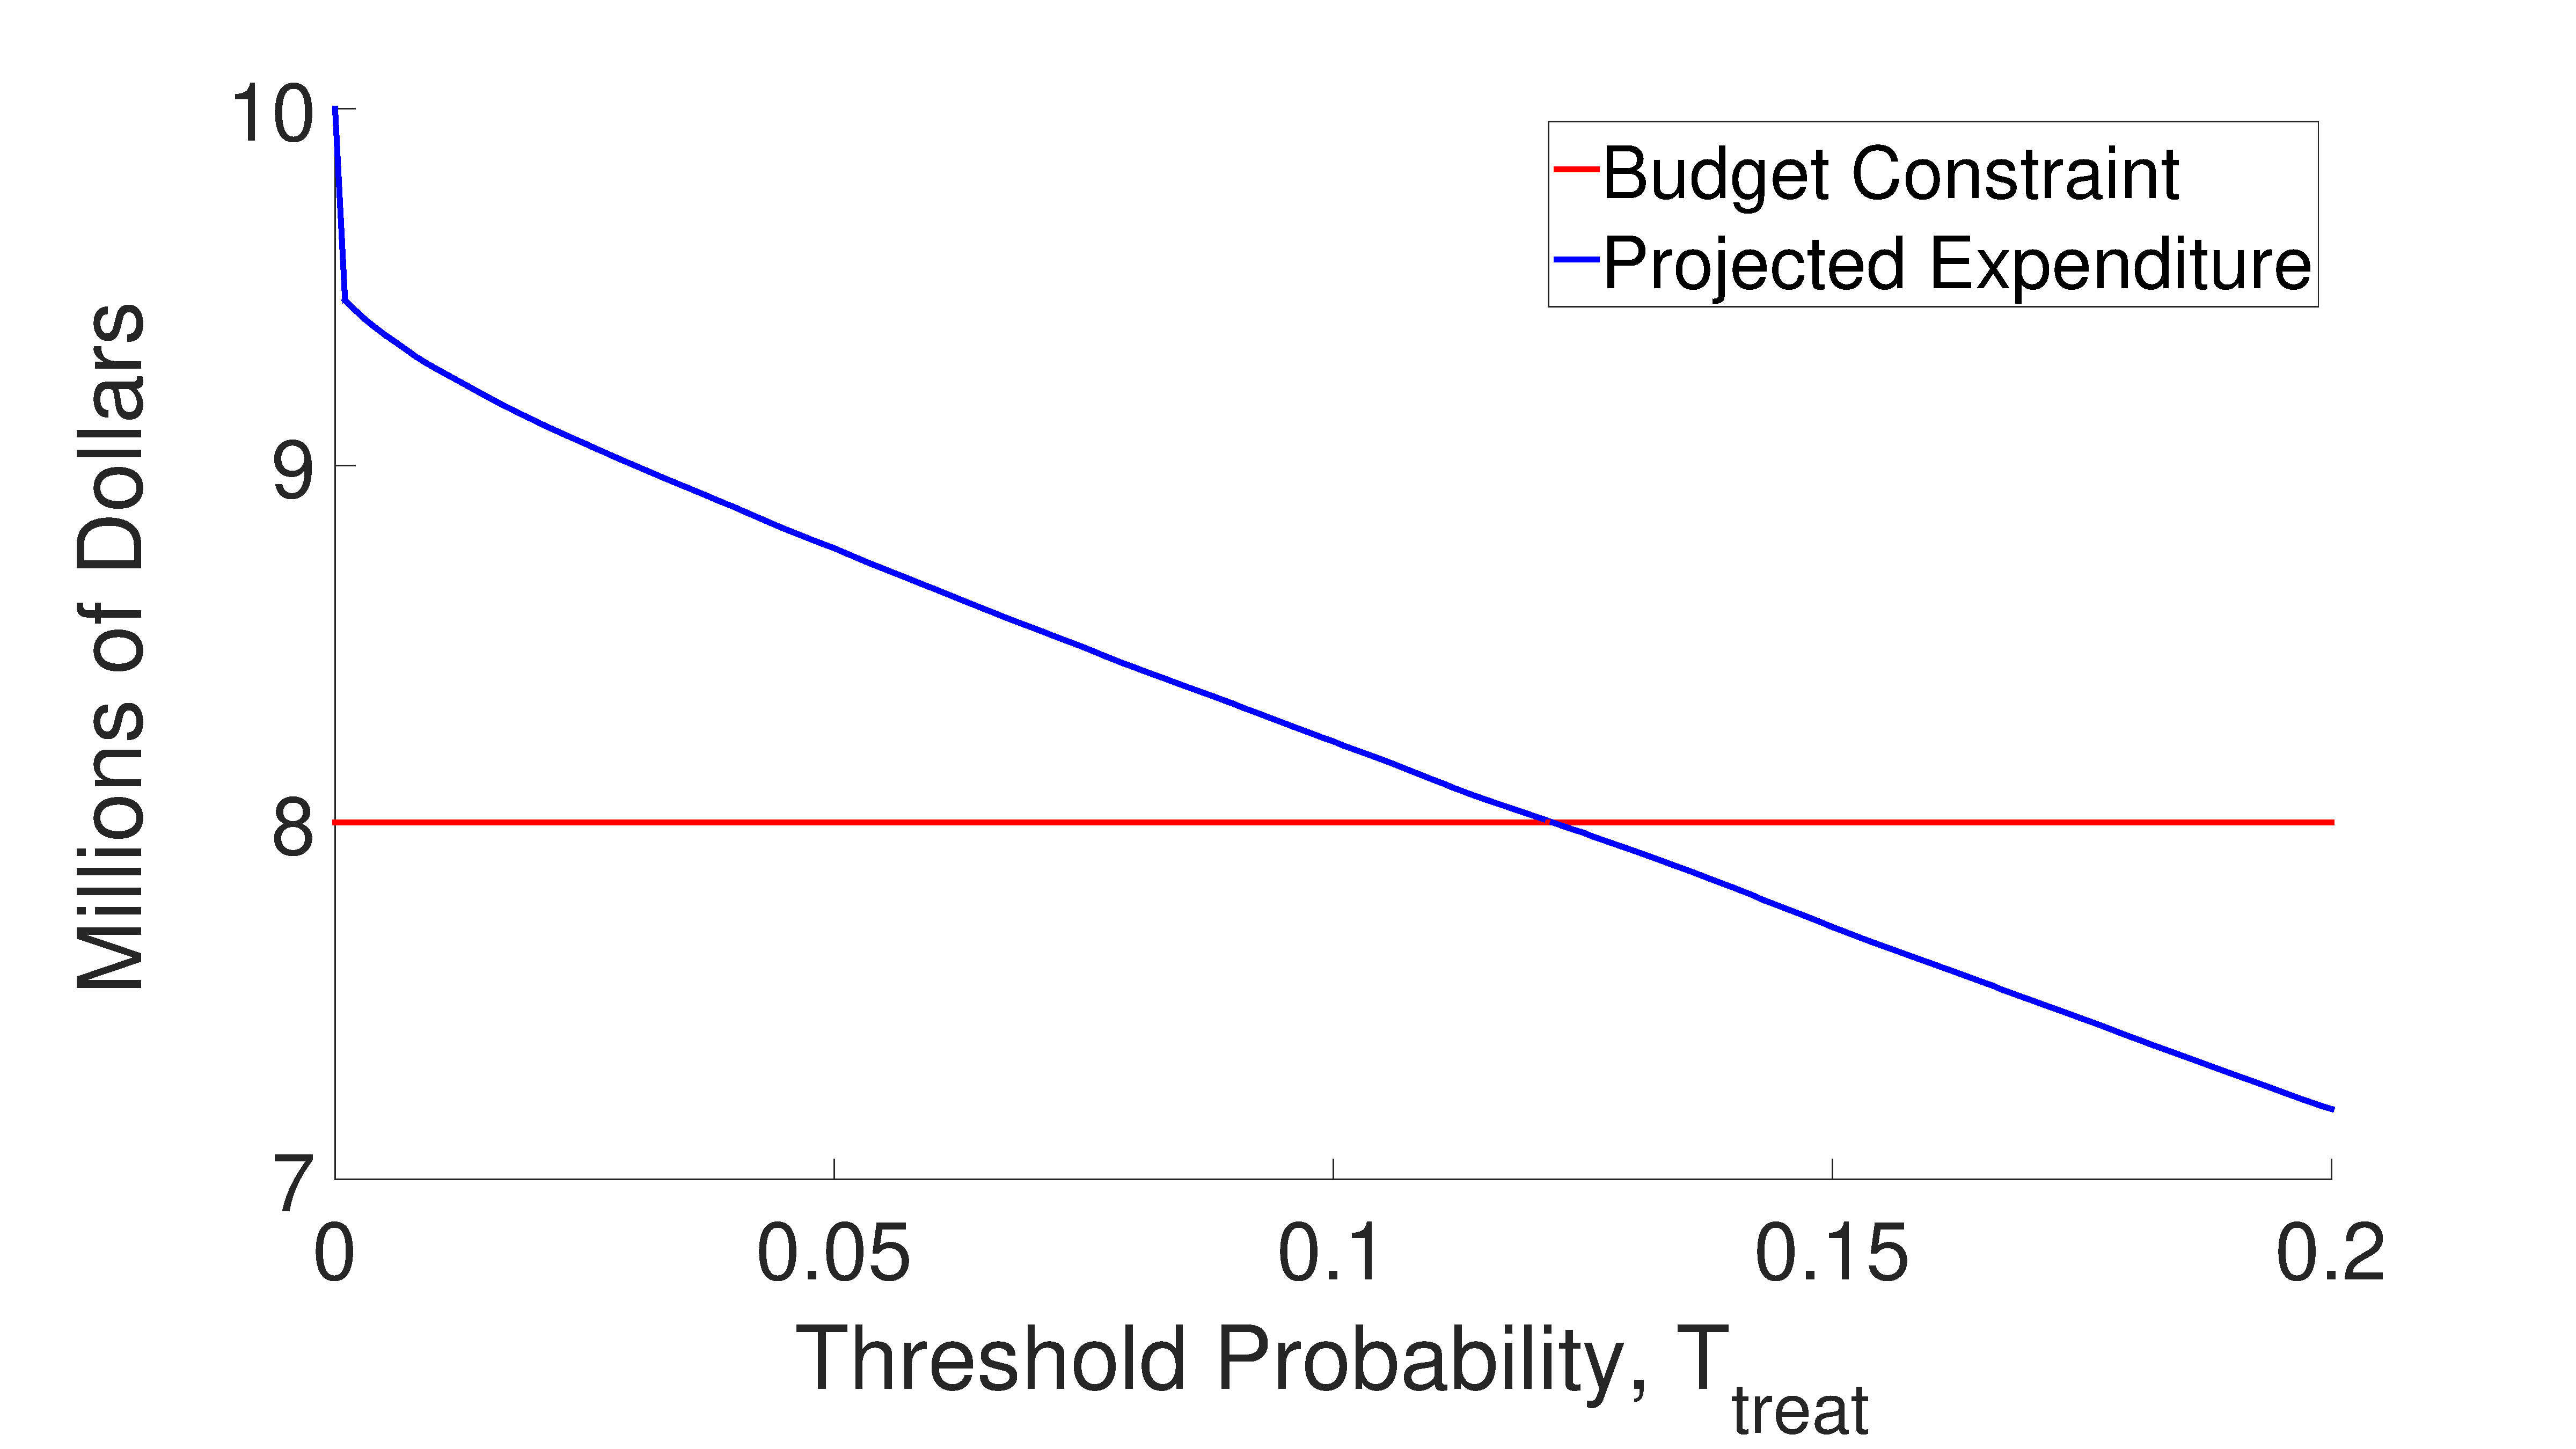
\includegraphics[width=0.48\textwidth]{budget}
	\caption{Projected expenditure (proportional to $I_{N,M}$) evaluated at different values of $T_{\mathrm{treat}}$. The budget constraint is shown by the horizontal red line. The optimal value of $T_{\mathrm{treat}}$ is found by the intersection 
		and occurs at $T_{\mathrm{treat}} = 12.5\%$. Evaluated was carried out at 100 $T_{\mathrm{treat}} \i$. Only the bottom 20\% is pictured as this is the operating range for most treatment centers. }
	\label{fig:emperical-cost}
\end{figure}

The model is completed by the definition of the following distributions and parameters.
\begin{align*}
& K_0 = 100000000, \quad
\phi = 0.001, \quad
\psi = 0.05, \quad
\lambda = 0.5, \quad
\xi \sim \text{Beta}(5, 2), \\
& c_0 \sim 1000*\text{Rayleigh}(10), \quad
T_{\text{opp}} = 2000,\quad
T_{\text{treat}} = 0.35, \quad
t_{\text{max}} = 250, \quad
t_{\text{step}} = 0.01 
\end{align*}

\subsection{Budget result}
\label{sec:cancer_sim_result}

In the example outlined above, the treatment center is not actually attempting to evaluate the value of $I$, but to find the optimal value of $T_{\text{treat}}$ subject to a budgetary constraint. A simplistic way of evaluating the optimal value is to perform a dense search over different values of the parameter, each time evaluating the estimated expenditure, and select the best performing value.

Figure~\ref{fig:emperical-cost} shows the variation of predicted expenditure against the threshold probability, as well as the budget constraint. The intersection of these curves is the optimal setting of $T_{opp}$, here evaluated to be 12.5\%. From the blue line, it is clear that the relationship between expenditure and treatment probability is non-linear, especially at the extrema of the distribution, and hence the use of NMC was necessarily for evaluating the optimal value. 


